\documentclass[10pt,letterpaper]{article}

\usepackage{cogsci}
\usepackage{pslatex}
\usepackage[nodoi]{apacite}
\usepackage{graphicx}
\usepackage[american]{babel}
\usepackage{amsmath}
\usepackage[section]{placeins}
\usepackage{enumitem}


\title{Beyond Na\"{i}ve Cue Combination: \linebreak Salience and Social Cues in Early Word Learning}
 
 \author{{\large \bf Daniel Yurovsky} \\ \texttt{yurovsky@stanford.edu}\\ Department of Psychology \\ Stanford University
	\And {\large \bf Michael C. Frank} \\ \texttt{mcfrank@stanford.edu} \\ Department of Psychology \\ Stanford University}

\begin{document}

\maketitle

\begin{abstract}

Children learn their earliest words through social \emph{interaction}, but it is unknown how much they use social \emph{information}. Some theories argue that word learning is fundamentally social from its outset, with even the youngest infants understanding intentions and using them to infer a social partner's target of reference. In contrast, other theories argue that early word learning is largely a perceptual process in which young children map words onto salient objects. One way of unifying these accounts is to model word learning as weighted cue-combination in which children attend to many potential cues to reference, but only gradually learn the correct weight to assign each cue \cite{Hollich2000}. We test 3 predictions of a na\"{i}ve cue-combination account and show each to be incorrect. Thus, while aspects of this unifying account are correct, it must be amended to capture the dynamics of children's behavior across differing referential situations.

\textbf{Keywords:} 
Language acquisition, word learning, attention, social cues, cognitive development
\end{abstract}


\section{Introduction}

% Predictions of Naive Cue Combination Accounts
% Cues should be normalized in some way, one shouldn't go up unless another goes down.
% same cues that matter in learning will matter at test
% When perceptual cues win early, they should draw attention. Face should be unimportant.
% 
% 

%How do young children learn the meanings of their first words? For example, when an adult produces a novel label in a complex natural scene, how can a child determine to which object---if any---the label refers \cite{Quine1960, Bloom2000}? For adults, this problem is straightforward; in addition to learning a language, adults have learned to consult a speaker�s social gestures and use their understanding of a speaker�s communicative goals \cite{Clark1983}. Social inference also characterizes the word-learning strategies of children late in their second year \cite<e.g,>{Baldwin1991, Brandone2007,Grassmann2010}. But word learning likely begins much earlier, perhaps as early as at 6-months \cite{Tincoff1999, Bergelson2012}. Do very young children use social information to reduce referential uncertainty in early word learning?

How do children learn the meanings of their first words? Infants are situated in a social system from their first day of life, and some theories argue that they leverage this social information from the very outset of word learning \cite{Bloom1998}. For instance, infants follow direction of gaze by 6-months \cite{D'Entremont1997}, and are more likely to do so in the presence of other communicative signals \cite{Senju2008}. Individual differences in children's gaze-follwoing predict differences in vocabulary development \cite{Brooks2008}. In addition, infants appear to representing others' beliefs, and these representations affect their expectations by 12-months of age \cite{Vouloumanos2012}. Infants are thus tuned to social cues and could in principle already use these cues from the outset of word learning.\footnote{For convenience we refer to ``word-object mapping'' and ``word learning'' interchangeably,  but acknowledge that referential mapping is only part of simple object-noun learning (the current case study). Generalization is unaddressed here.}

Yet some competing theories argue that early word learning is primarily a perceptual process \cite{Vygotsky1978} and that infants learn words by mapping them onto salient objects in their learning environments \cite{Smith2000}. Indeed, early child-directed naming events are characterized by multi-modal synchrony: mothers move the objects they label in temporal synchrony with the labels they speak \cite{Gogate2000}, and the degree of synchrony predicts mapping for young infants \cite{Gogate2006}.

To unify these views, \citeA{Golinkoff2006} proposed the \emph{Emergentist Coalition Model}. From this perspective, children are sensitive to a coalition of cues-to-reference: both perceptual cues like visual salience and temporal synchrony, \emph{and} social cues like eye-gaze and pointing. To determine the referent of a speaker's utterance, children \emph{combine} all of the available cues. However, the weights assigned these cues are fixed, but change over the course of development as children learn which cues are the best predictors of reference. Early on, children are biased to assign high weight to perceptual cues, but as they learn that social cues are better predictors, they gradually weigh them more.

Support for a developmental cue-combination account comes from studies that pit perceptual salience against social information (e.g., speaker gaze) at different developmental ages. When social gaze conflicts with perceptual salience, 10-month-old infants show no evidence of attending to gaze \cite{Pruden2006}. Although 10-month-old infants may be able to follow gaze, they appear to weigh it significantly less than object salience in mapping words to objects. Under similar conditions, 12- and 15-month-olds fail to learn any mappings \cite{Hollich2000, Houston-Price2006}. By 19- and 24-months, however, toddlers learn labels for objects cued by gaze even in the presence of salient competitors \cite{Moore1999, Hollich2000}. 

Weighted cue-combination is an intuitive, computationally simple model of the process of change in early word learning \cite{Frank2013a}, and it is consistent with properties of our perceptual system \cite{Ernst2002, Jacobs2002}. Within and across modalities, adults weigh cues in proportion to their predictive power, combining them as predicted by ideal observer models. Yet, in the domain of early word learning, a number of its detailed predictions remain untested. 

Using eye-tracking to measure early word learning from social information, we test three predictions of the cue-combination model of developmental change:

\begin{enumerate}[noitemsep]
	\item Developmental change is due to re-weighting across cues,
	\item Cue weights drive attention during learning, and
	\item Perceptual cues decrease in weight across development.
\end{enumerate}

\noindent Two experiments show that none of these predictions are correct. Thus, while cue-combination captures important insights about early word learning, a na\"{i}ve version of this account is insufficient.

\begin{figure*}[t]
	\center{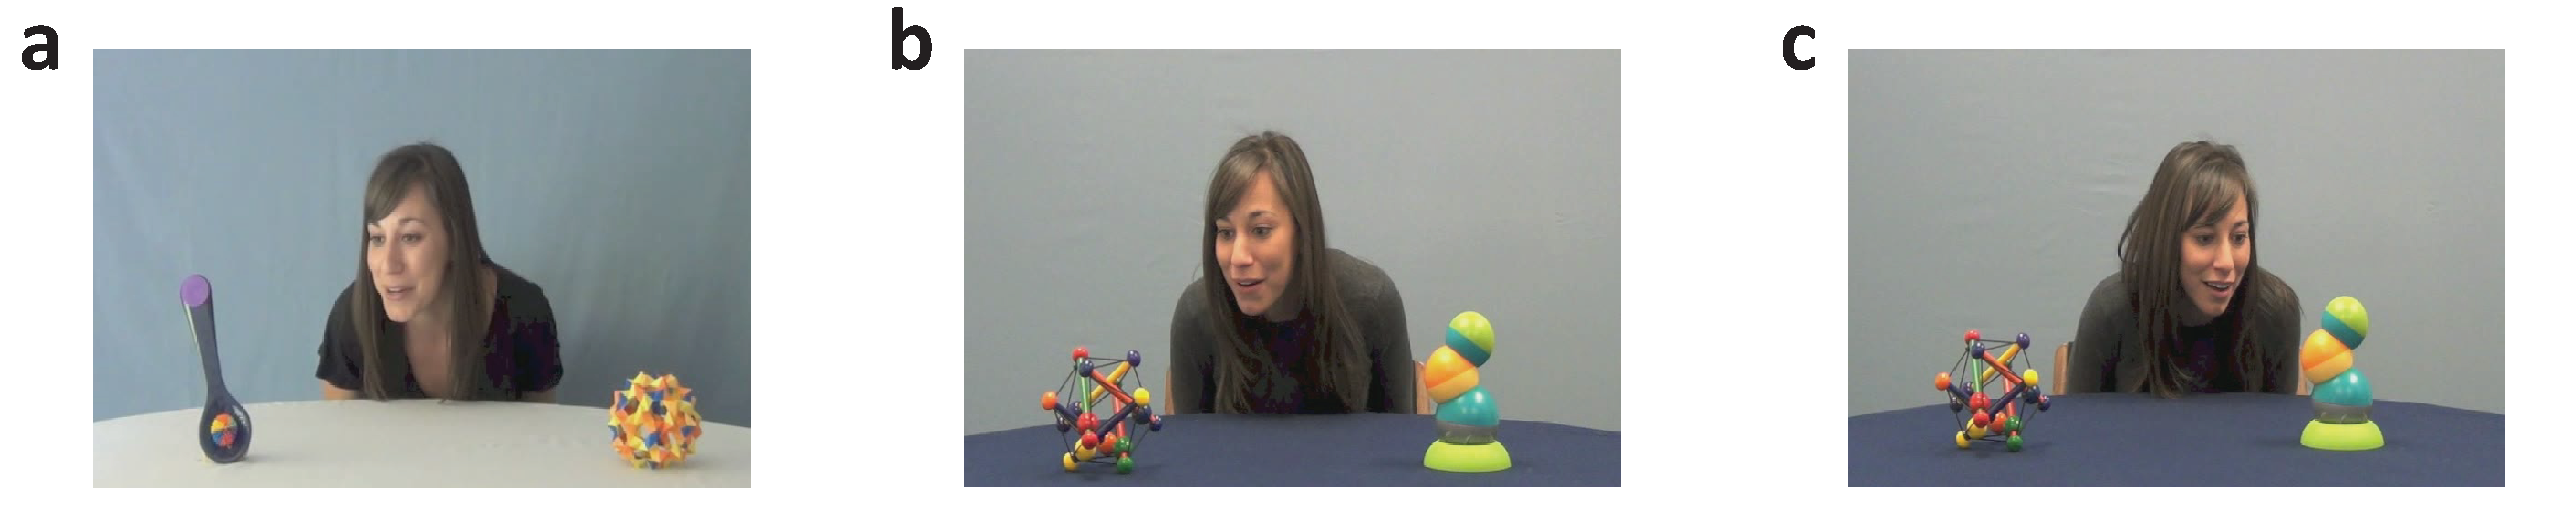
\includegraphics[width=\textwidth]{figures/tri_fig.pdf}}
	\caption{\label{fig:design} Example learning trials from Experiments 1 and 2. In Experiment 1 (a), the speaker turned towards one of the equally-salient toys and labeled it three times over the course of approximately 10 seconds. In Experiment 2, the speaker produced the same social cues and the same label as in Experiment 1, but the target object was either the more perceptually salient toy (b), or the less perceptually salient toy (c). These manipulations allow measurement of the contributions of both salience and social information to word-object mapping.}
\end{figure*}

\section{Experiment 1}

In Experiment 1, we set out to measure the development of children's ability to follow and learn from social gaze in the absence of competing salience cues. A na\"{i}ve cue-combination account, in which developmental changes in cue use result from learning their relative predictive weights, makes a null prediction: children's behavior should not change significantly across development. 

Children's eye movements were tracked while they watched a series of naturalistic word-learning videos. In each, children saw a speaker seated at a table between two novel toys. She greeted them, and then turned towards one of the toys and labeled it three times in a short monologue.
After these learning trials, children were tested for their knowledge of the referent for the new word using the preferential looking procedure. In addition, to measure children's processing abilities for familiar words, similar test trials were administered with known items.

\subsection{Method}

\subsubsection{Stimulus Norming}
Thirty-eight adult participants on Amazon Mechanical Turk were presented two toys at a time, from a set of 10, and asked to select the one they would rather play with. Each participant made 20 such choices, with toys sampled at random, producing ~7.6 responses for each pair of toys. Based on these responses, we selected the two toys that were best balanced against each other (see Figure~\ref{fig:design}a).

\subsubsection{Participants}

Parents and their 1--4 year-old children were invited to participate in a short language learning study during their visit to the San Jose Children's Discovery museum. In total, we collected demographic and experimental data from 269 children, 122 of whom were excluded for one or more of the following reasons: abnormal developmental issues ($N= 27$), failure to calibrate ($N=58$), and less than 75\% exposure to English ($N=36$). The final sample consisted of 27 1--1.5 year olds (9 girls), 19 1.5--2 year olds (7 girls), 38 2--2.5 year olds (13 girls), 26 2.5--3 year olds (10 girls), 15 4--3.5 year olds (9 girls), and 22 3.5--4 year olds (11 girls).

\subsubsection{Stimuli and Design}

The experiment consisted of two kinds of trials designed to measure both how children allocate their attention while learning from a social partner, and what word-object mapping information they extract from these learning events. Learning trials were ~12s video clips in which a speaker first greeted the the child, and then turned towards one of the two toys on the screen, labeling it three times in a short monologue (Figure~\ref{fig:design}a). On the first learning trial, for example, the speaker said ``Hi there! It's a \emph{modi}. Look at the \emph{modi}. What a nice \emph{modi}.''

On each test trial, children saw two objects---one on each side of the screen---and heard a short audio clip of the speaker from the learning trials asking them to find a target object. Each test trial was 7s long, and the target label was heard at ~2.75s. On \emph{Familiar} test trials, both the target and competitor were common objects familiar to young children (e.g. book vs. dog). On \emph{Novel} and  \emph{Mutual Exclusivity (ME)} test trials, children saw both of the toys from the previous learning trials, and were asked to find either the previously named toy (\emph{modi}), or were asked about a novel label (\emph{dax}). These ME trials were designed as a strong test of mapping formation; looking to the correct target on Novel trials could result from familiarity or preference rather than mapping. However, correct performance on both Novel and ME trials could only result from knowledge of the specific label used in training.

Finally, the experiment contained two calibration checks: short videos in which small dancing stars appeared in four places on the screen. These checks allowed us to adjust initial calibration settings to when they were imprecise \cite<for details, see>{Frank2012d}.


\subsubsection{Procedure}

The eye-tracker was first calibrated for each child using a 2-point calibration. Next, children saw four learning trials in which the speaker produced the novel label and disambiguated her target of reference with social gaze. Finally, children saw all of the test trials, in which their knowledge of both familiar and novel word-object mappings was tested. Two calibration checks (described above) were embedded in the learning phase. The entire experiment consisted of 4 learning trials, 8 Familiar, 6 Novel, and 6 ME test trials.

\subsubsection{Data Analysis}

Children's eye movements during both learning and testing were analyzed using a Regions of Interest (ROI) approach. Bounding-box ROIs were drawn by a human coder for the speaker's face (learning trials) and for the two objects (learning and test trials). Children's calibrations were adjusted by fitting a robust linear regression for their fixations during calibration check videos and using this model to transform eye movements during the rest of the experiment \cite{Frank2012d}.

Children's learning and test behaviors were quantified by measuring their proportion of looking to each ROI on each trial. To ensure that proportions were representative, individual test trials were excluded from analysis if eye gaze data was missing for more than half of their duration. To compute age-group looking proportions, proportions were computed first for each individual trial, averaged at the individual-child level, and then averaged across children.

Window-of-analysis selection began by coding the point of disambiguation for each trial. This was the onset of the target label for test trials, and the rotation of the speaker's head for learning trials. The window for each trial began 1s after this point of disambiguation to allow children of all ages enough time to process and continued out to 3s after this point on both learning and test trials. To quantify learning with standard analyses, we aggregated these patterns of looking over time to compute proportion of target looking on each test trial. 

\subsection{Results}

In Experiment 1, we address two predictions of na\"{i}ve cue combination: how cues affect attention during learning, and how weights change across development.

\subsubsection{Older children were better at \emph{disengaging} from social stimuli} 

Children were successful at attending to and following the speaker's social gaze even from the youngest ages measured. Children of all ages spent more time looking at the target than at the competitor during learning trials (smallest $t(23)  = 3.20$, $p < .01$). However, for all age groups, looks to both target and competitor made up the minority of children's dwell times. Instead, children in all age groups spent more than 50\% of their time attending to the speaker's face (Figure~\ref{fig:exp1_train}).\footnote{All data and code for analysis available at \small{\tt{http://github.com/dyurovsky/ATT-WORD}}.} Thus, the primary driver of developmental change was not stronger discrimination between the target and competitor (predicted by greater social cue weights), but rather improved ability to disengage from the speaker's face. 

 \begin{figure}[t]
	\center{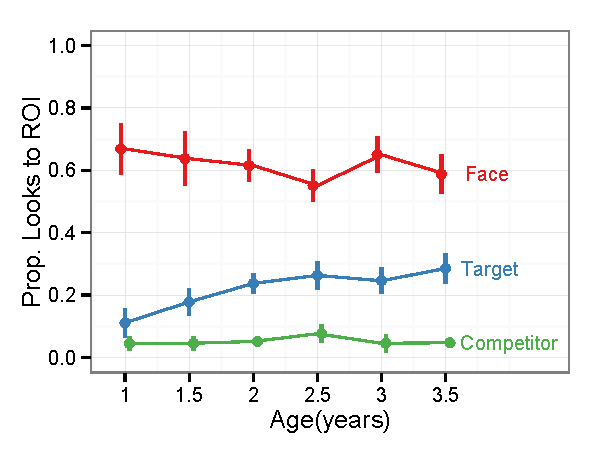
\includegraphics[width=.5\textwidth]{figures/exp1_train.pdf}}
	\caption{\label{fig:exp1_train} Proportion of children's looking the target toy, competitor toy, and the speaker's face during learning in Experiment 1. Children of all ages spent the majority of the learning trials looking at the speaker's face. Disengaging from the face and fixating the target increased across development. Error bars indicate 95\% confidence interval computed by non-parametric bootstrap.}
\end{figure}

\vspace{9 pt}

\subsubsection{Developmental change was not primarily due to re-weighting.} 

In line with the na\"i{v}e cue combination account, attention due to the social cue during learning carried forward to correct mapping at test. Analyses of test trials showed broad success on Familiar, Novel, and ME trials across development. The 1--1.5 year-olds trended towards significance on familiar trials ($t(26)  = 1.65$, $p = .11$), and were non-significantly in the correct direction on Novel and ME trials. At all other ages, children looked to the target at above-chance levels on all test trials (smallest $t(17)  = 2.10$, $p = .05$). 

However, children's abilities both to follow social cues during learning trials and to find the correct target on test trials improved across development. To quantify this improvement, we fit a mixed effects logistic regression to the data \cite{Jaeger2008}. This analysis revealed significant improvement across age ($\beta = .61$, $z = 4.03$, $p <.001$), as well a significant significant effect of Learning as compared to Novel trials ($\beta = 1.18$, $z = 3.11$, $p <.01$). No other effects or interactions approached significance. Figure~\ref{fig:exp1_train_test} shows proportion of looking all kinds of trials at all ages. 

Thus, across development, children improved in learning from the social cue, even when it was the only cue available. This suggests that re-weighting across cues is not the only driver of improved word learning.

\begin{figure}[!t]
	\center{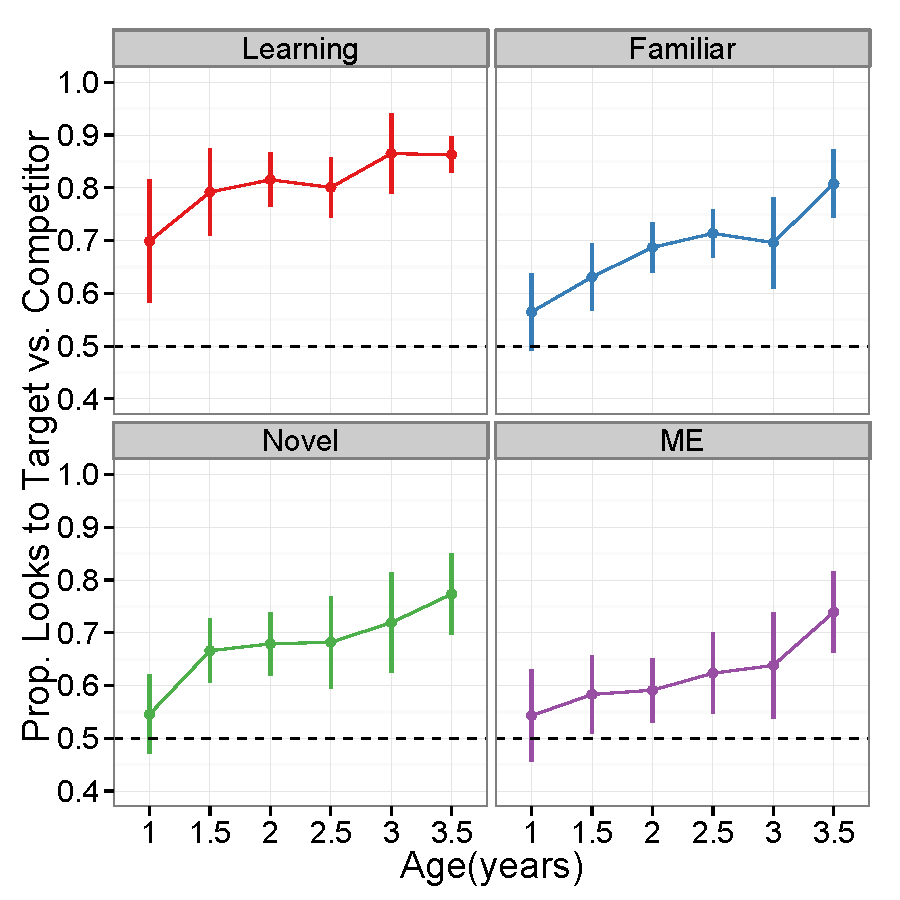
\includegraphics[width=.45\textwidth]{figures/exp1_train_test.pdf}}
	\caption{\label{fig:exp1_train_test} Proportion of time children fixated the correct correct target on each type of test trial in Experiment 1. Children improved on all measures across development. Each dot indicates one half-year age group and each line represents a 95\% confidence interval computed by non-parametric bootstrap. A proportion of .5 indicates chance performance.}
\end{figure}	

\subsection{Discussion}

Together, these results provide evidence both of early competence in the use of social gaze to determine the target of a speaker's reference, as well as improvement across development. Further, improvements in gaze-following also paralleled improvements in both finding the referents of these novel words on subsequent test trials, and also finding the referents of familiar words (Figure~\ref{fig:exp1_train_test}).

These results thus provide support for one key claim of the developmental cue-combination account: children are sensitive to social cues quite early. Young children could assign small---but non-zero---weight to social cues, and then gradually assign them more credibility over development. However, the results also provide evidence \emph{against} the prediction that cues drive attention, and that developmental change is due to relative re-weighting for two reasons. First, children of all ages found the speaker's face highly engaging, and spent the majority of their time fixating it rather than the referents on learning trials. The primary behavioral development was the ability to disengage from the speaker's face. Second, children showed gradual improvement in fixating the target during both learning and test trials well into their fourth year.

This data could be consistent with a modified version of the cue-combination account in which cues both change in both their absolute and relative weights due to learning. However, while children undeniably encounter naming events in their third and fourth years, it seems unlikely that the process of learning the cue validity of social gaze would extend over such a long period of time. 

In Experiment 2 we manipulated the relative salience of the target and competitor objects children learned about. This allowed us to measure how salience affects children's looking during both learning and test, providing a test of all three predictions of the na\"{i}ve cue-combination account.

\section{Experiment 2}

Experiment 2 was identical to Experiment 1 in all respects except for the identity of the novel toys that served as the target and competitor. In contrast to Experiment 1, in which the two toys were balanced in their visual salience, the two toys in Experiment 2 were mismatched. For children in the \emph{Salient} condition, the target was the more interesting toy, and the competitor the less interesting toy. In the \emph{Non-Salient} condition, the identities of the toys were switched---the target was the less salient toy. Thus, Experiment 2 allowed us to investigate children's use of social cues to learn new words when they are aligned with salience, and when they were in opposition \cite<as in>{Hollich2000,Pruden2006}.

\subsection{Method}

\subsubsection{Participants}

Participants were recruited from the floor of the San Jose Children's Discovery museum as in Experiment 1. For Experiment 2, we focused on the three youngest age groups. In the Salience condition, demographic and experimental data were collected from 117 children, 52 of whom were excluded for one or more of the following reasons: abnormal developmental issues ($N= 13$), failure to calibrate ($N=25$), less than 75\% exposure to English ($N=33$), and inattentiveness ($N=2$). The final sample consisted of 22 1-1.5 year olds (11 girls), 21 1.5-2 year olds (10 girls), 19 2-2.5 year olds (9 girls). In the Non-Salience condition, data were collected from 126 children, 71 of whom were excluded for one or more of the following reasons: abnormal developmental issues ($N= 9$), failure to calibrate ($N=26$), and less than 75\% exposure to English ($N=36$). The final sample consisted of 26 1-1.5 year olds (13 girls), 25 1.5-2 year olds (11 girls), 15 2-2.5 year olds (4 girls).

\subsubsection{Stimuli, Design, and Procedure}

Experimental stimuli were identical to those in Experiment 1, except that the identities of the novel toys were changed and new videos were recorded. The procedure, including the order of the trials, was identical.

\subsection{Results and Discussion}
\begin{figure}[!t]
	\center{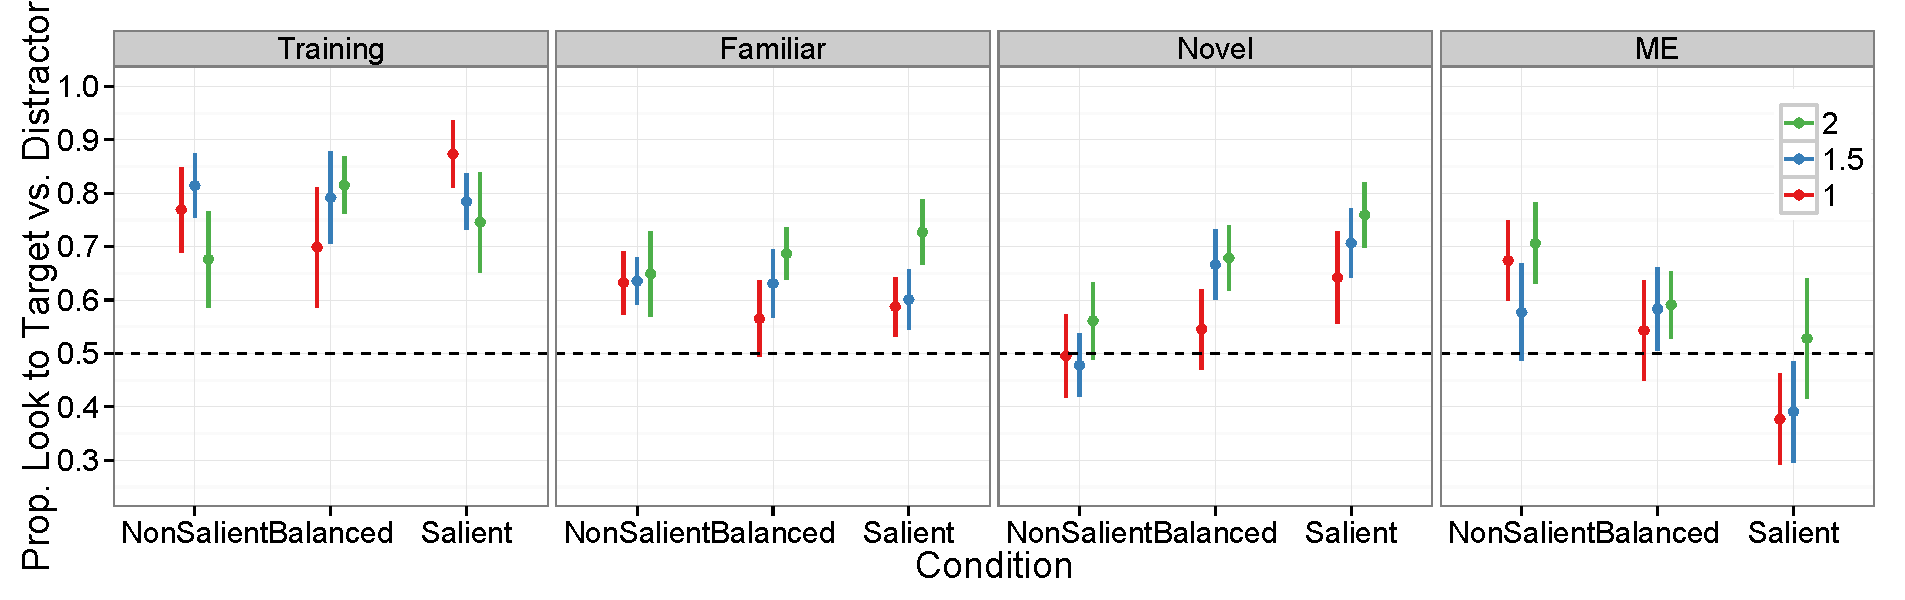
\includegraphics[width=.45\textwidth]{figures/exp1_2_train_test.pdf}}
	\caption{\label{fig:exp1_2} Proportion of time children fixated the correct correct target on Learning and Test trials in Experiments 1 (three youngest age groups) and 2. Salience had the predicted effect on looking behavior at test, but relatively little during learning. Each dot indicates one half-year age group and each line represents a 95\% confidence interval computed by non-parametric bootstrap. A proportion of .5 indicates chance performance.}
\end{figure}

\begin{table}[!b]
\begin{center} 
\caption{Mixed-effects Regression Coefficients Predicting Looking Behavior in Experiments 1 and 2.} 
\label{tab:model_table} 
\vskip 0.12in
\begin{tabular}{l r r r l} 
\hline
Predictor  &  Value (SE) & \emph{t}-value & Sig.\\
\hline
Intercept  & -.65 (.63) & -1.04 & $p = .3$&\\
Age (yrs) & .42 (.27) &  1.58 & $p = .11$&\\
Familiar & 1.55 (.73) & 2.13 & $p < .05$&*\\
Salient  & .96 (.48) & 1.98 & $p < .05$&*\\
NonSalient  & -.97 (.37) & -2.63 & $p < .01$&**\\
Learning & 1.55 (.73) & 2.13 & $p < .05$& *\\
ME & -.29 (.36) & -.80 & $p =.42$&\\
Salient*Learn  & -.03 (.84) & -.035 & $p = .97$&\\
NonSal*Learn & 1.09 (.65) & -1.65 & $p = .85$&\\
Sal*ME & -2.28 (.61) & -3.73 & $p = -.09$&.\\
NonSal*ME  & 1.67 (.54) & 3.07 & $p < .01$&**\\
\hline
\end{tabular} 
\end{center} 
\end{table}

To determine the effect of perceptual salience on word learning, we compared children's looking in the Salient and Non-Salient conditions not only to each other, but also to the Balanced condition in Experiment 1. 

\subsubsection{Perceptual salience did not drive attention during learning.} 

In contrast to the prediction of the na\"{i}ve cue-combination account, children's looking behavior during learning trials was not significantly affected by the salience of the target and competitor (Figure~\ref{fig:exp1_2}, top). As in Experiment 1, children of all ages spent the more time looking at the target than the competitor, but looking time to both made up the minority of their dwell time; children spent the majority of learning trials looking at the speaker's face.

This null-result could be due to the toys being too similar in their salience, making this a weak test of the cue-combination model. However, salience exerted a strong effect on test trials---children in all age groups were strongly attracted to the salient object. When the target referent was salient, children at all ages looked at it for the majority of the window of analysis on Novel test trials (smallest $t(19)  = 2.96$, $p < .01$). When the target was non-salient, no age group look showed evidence of learning on Novel test trials (largest $t(13)  = 1.46$, $p = .17$). Mutual-exclusivity (ME) trials showed the opposite pattern. When the target referent was salient, children in the two younger age groups looked at the correct referent on ME trials (the competitor) at \emph{below} chance levels (smallest $t(20) = -2.29$, $p < .05$). In the Non-Salient condition, even the youngest children looked at the correct referent on ME trials at above chance levels (smallest $t(22) = 4.51$, $p < .001$). Figure~\ref{fig:exp1_2}, middle/bottom) shows looking behavior at test in both Experiments 1 and 2.

\subsubsection{Perceptual cues did not decrease in weight across development.}

The effect of perceptual cues at test did not appear to change across development. We fit a mixed-effects logistic regression to the data from all three experiments to determine how how age and experimental condition impacted looking behavior in training and test. After controlling for performance on Familiar trials, this regression showed a significant effect of condition, and an interaction between trial type and condition. Children looked more to the salient object at test regardless of whether it was the target or competitor, and significantly more at the target during learning trials regardless of whether it was salient. Further, there was none of these factors interacted with age (Table~\ref{tab:model_table}). 

\subsubsection{Developmental change was not due to re-weighting across cues.} 

Together with the t-tests above, this analysis suggests that children are not relatively re-weighing salience and social cues over the course of development. While salience certainly plays a role in directing looking behavior, it does not appear to play a role during learning itself. Instead, salience appears to have a strong effect during test. In the absence of any social information, salience directs children's attention in a way that does not appear to change over early development.

\section{Conclusion}

Is children's early word-object mapping fundamentally social, or is it mostly driven by perceptual processes? A weighted cue-combination account provides a simple framework to unify social and perceptual factors in early word learning \cite{Hollich2000, Frank2013a}. Under this kind of account, perceptual cues are weighed higher in early learning, while social cues gradually gain weight as children learn their predictive power over early development. We tested this account in two word-learning experiments and found that its predictions were inconsistent with the data. 

Although a cue-combination account would predict that developmental change is largely driven by the relative re-weighting of cues, our data showed little evidence of this (contra prediction 1). Instead, developmental changes during learning appeared to be driven by disengagement from the social stimulus, not disengagement from the perceptually salient target (contra prediction 2). Finally, perceptual salience exerted its effects mostly at test, and did so continuously across early development instead of declining in weight (contra prediction 3). 

Learning a new word relies on processes that work at multiple time-scales: children need to identify a speaker's referent in-the-moment, encode a mapping between the label and referent, recall multiple labeling events and integrate across them, and use their learned mappings to identify the object in novel contexts \cite{McMurray2012, Yu2012b}. Na\"{i}ve cue-combination is too simple a model because it does not distinguish among these component problems. In these experiments, for instance, children used different cues to identify a speaker's referent and to find it in a novel test context. Building a more satisfying model of the developing word learning will require integrating the cues children use to identify referents with an understanding of how these cues interact with attentional control, memory, and the conversational contexts in which naming occurs \cite{Frank2013a, Yurovsky2013c}. 

\section{Acknowledgments}

We are grateful to Janelle Klaas for collecting the data, and to  all of the members of the Language and Cognition Lab for their feedback on this project. In addition, we thank the parents, children, and staff at the San Jose Children's Discovery Museum for supporting us in collecting developmental data. This work was supported by a NIH NRSA F32HD075577 to DY as well as grants from the Merck Scholars Foundation and the Stanford Center Health Research Initiative to MCF.

\bibliographystyle{myapacite}

\setlength{\bibleftmargin}{.125in}
\setlength{\bibindent}{-\bibleftmargin}

\bibliography{library11}


\end{document}
